\begin{figure} [htb!]
    \centering
    % feel free to improve this i don't actually know how to use this
    \tikz{
        % nodes
        \node[obs] (y) {$\rx$};%
        \node[latent,left=of y, xshift=-.4cm] (z) {$\rz$} ; %
        \node[obs,left=of z, xshift=-.4cm] (w) {$\rw$}; %

        % Factors
        \factor[left=of y, xshift=-.2cm] {z-y} {below:$\pld{x\given z;y}$} {} {} ; %
        \factor[left=of z, xshift=-.2cm] {w-z} {below:$\pld{z\given w}$} {} {} ; %

        \factor[above=of z, yshift=.1cm] {q} {above:$\qvd{z\given x,w;y} \approx \pld{z\given x,w;y}$} {} {} ; %
        \factor[below=of z, yshift=-.1cm] {r} {below:$\rvd{w\given x;y} \approx \pld{x\given w;y}$} {} {} ; %

        \node[const,above=of y, yshift=-.42cm] (y_above) {} ;
        \node[const,below=of y, yshift=.42cm] (y_below) {} ;
        \node[const,above=of w, yshift=-.42cm] (w_above) {} ;
        \node[const,below=of w, yshift=.42cm] (w_below) {} ;
        
        % % plate
        % \plate [inner sep=.25cm,yshift=.2cm] {plate1} {(x)(y)(z)} {$N$}; %
        % edges
        % \edge {w} {wt} ;
        % \edge {wt} {z} ;
        % \edge {z} {y} ;

        \edge[dashed, -] {w} {w_above} ;
        \edge[dashed, -] {y} {y_above} ;
        \edge[dashed] {w_below} {w} ;
        \edge[dashed, -] {y} {y_below} ;
        
        % factor edges
        % \factoredge[densely dashdotdotted] {w} {w-wt} {wt} ; %
        % \factoredge[densely dashdotdotted] {wt} {wt-z} {z} ; %
        \factoredge {w} {w-z} {z} ; %
        \factoredge {z} {z-y} {y} ; %

        \factoredge[dashed] {w_above,y_above} {q} {z} ; %
        \factoredge[dashed,-] {y_below} {r} {w_below} ; %
    }
    \caption{Overview of the probabilistic formulation for the proof of concept, with context $\ry$ omitted for clarity, showing where each of the variational approximations fit into the overall picture.}
    \label{fig:wzx-poc}
\end{figure}


As outlined in \cref{sec:intro-variants}, we will first need to learn posterior distributions $\pld{z\given x,w;y}$, while simultaneously fitting our model to historical observations. Then, we can use this learned model to predict effects of different conditions on a new day, or learn a different conditional density of interest. To this end, we apply stochastic variational inference, as introduced in \cref{background-variational-inference}, for the same reasons of computational tractability. In \cref{fig:wzx-poc}, we outline the distributions we are attempting to approximate. 

\subsection{Cluster Labels}

We will start with learning an approximation for latent posterior distribution $\qvd{z\given x,w;y}\approx \pld{z\given x,w;y}$. As discussed in \cref{sec:atrds-single-airport}, it is difficult to immediately identify which data points to group together for accurate learning of separate posteriors, so we will also learn a way to simultaneously cluster these points into groups, in a principled way, which also effectively also makes part of our learning problem unsupervised.

For this case study, we also adopt a simple threshold-based classification model. Specifically, we also select thresholds $\xth$ and $\yth$, and define a clustering function $\gvn:(x,y,w)\mapsto (d_x,d_y,d_w)=d$ as follows, with $x'$ and $y'$ as the result from aggregating $x$ and $y$ as described in \cref{sec:atrds-single-airport}:
\begin{proposition}[Partial Relaxation of Clustering for $\gvn$]
    We define our clustering function $\gvn$ as follows:
    \begin{align}
        \gvd{x,y,w}_x = d_x &= \mbm1_{x'\ge\xth}\\
        \gvd{x,y,w}_y = d_y &= \mbm1_{y'\ge\yth}\\
        \gvd{x,y,w}_w = d_w & = 1 - \sigma\left(\alpha (w_v-\wthvg)\right)\cdot \sigma\left(\alpha (w_c-\wthcg )\right) \\
        &\approx \begin{cases}
            1 \;\; \text{if} \;\; w_v \leq \wthvg \;\; \text{or}\;\;  w_c \leq \wthcg \\
            0 \;\; \text{otherwise.}
        \end{cases}
        % \begin{cases}
        %     1 \quad\text{if }\widetilde{x} \le\xth\\
        %     0 \quad{\text{otherwise}}
        % \end{cases}
    \end{align}
\end{proposition}

Here, $\mbm1$ is an indicator that takes on value $1$ when the condition is true and $0$ otherwise, and $\sigma(\cdot)$ is the sigmoid function.We use separate thresholds for the $w$ components in $\fvn$ and $\gvn$ because it is possible that the relevant thresholds for weather are different when also introducing contributions from other variables such as $y$. Similarly to $\fvn$, we set the parametrization for $\gvn$ as $\lambda = (\wthvg, \wthcg)$. In both $\fvn$ and $\gvn$, we use a smooth approximation for the weather threshold indicator to maintain differentiability, so the relevant ranges here are $c\in\ms C=[0,1]$ and $d\in \ms D=\{0,1\}\times \{0,1\}\times [0,1]$, where the $\times$ used here is the Cartesian product. 

By also learning this clustering, we can make sure that we are learning cleaner posteriors than if we had specified one beforehand that may or may not have been useful or just tried to learn on the entire dataset. It also allows us to perform amortized inference, because instead of just learning posteriors for our whole dataset $\Data$ or separate partitions of it, we instead learn separate posteriors conditioned on $d=\gvd{x,y,w}$ and the clustering function $\gvn$ at the same time, which means we can reuse our work and map new data points to a value of $d$ and use the relevant learned posterior, instead of having to do the learning process all over again.

It is also important to emphasize the difference between the cluster labels $d$ and the weather labels $c$, as they may appear to be the same at first glance. In particular, $c$ only depends on weather, and is only used in the forward direction of the $w\to z\to x$ model, so to speak. In contrast, $d$ depends on the entire data point $(x,y,w)$, and is used as a lower-dimensional label the learned posterior approximation $\qvn$ will be conditioned on.


\subsection{Variational Inference Setup}

Before we incorporate the labels $c$ and $d$, we will return to the general setting as shown in \cref{fig:wzx-poc} for a moment. Our problem differs somewhat from the standard variational inference setting, so we will provide derivations specific to our case for clarity. 

We assume $\rx,\rz,\rw$ are drawn from some true distribution $\ptd{\cdot;y}$, and we only have observations for $\rx$ and $\rw$. Then, as before, we let $\pld{\cdot;y}$ represent the learned model, in which we specify in two separate components for before and after the latent variable $\rz$.

In particular, $\pld{x\given z;y}$ may be specified by the simulated system dynamics, and $\pld{z\given w}$ by a specified model of the effect of weather conditions on the latent simulation parameters $z$. One benefit of this division is that dealing with the individual parts can be easier than trying to work with $w\to x$ directly, especially when the actual connection is not particularly clear, such as in our case.

Another benefit is that we immediately obtain a connection to the standard generative modeling setting by considering the relationship between individual parts of our model. Examining the joint distribution $\pld{x,z\given w;y}$, which may readily be rewritten as the product $\pld{x\given z;y}\pld{z\given w}$, a natural interpretation arises by considering the system dynamics of the simulation $\pld{x\given z}$ to be a standalone process, which uses weather-informed priors on the latent variables $\rz$ specified by $\pld{z\given w}$. However, it is important to note that while these specifications may be helpful in smoothly integrating domain knowledge into the model, it is not actually necessary to specify them, and our framework also encompasses a fully black-box treatment, as long as sufficient training data is available.

\begin{example}[Assortment of Conditional Densities]
    Here are some conditional densities obtained via Bayes' rule.
    \begin{align}
        \pld{x,w\given z;y} &= \pld{x\given z;y}\pld{w\given z}\\
        \pld{z,w\given x;y} &= \pld{w\given z}\pld{z\given x;y}\\
        \pld{x,z\given w;y} &= \pld{x\given z;y}\pld{z\given w}\\
        \pld{w\given x,z;y} &= \pld{w\given z} \\
        \pld{x\given z,w;y} &= \pld{x\given z;y} \\
        \pld{z\given x,w;y} &= \frac{\pld{x\given z;y}\pld{z\given w}}{\pld{x\given w}} = \frac{\pld{w\given z}\pld{z\given x;y}}{\pld{w\given x;y}}.
    \end{align}
\end{example}

Now, under this structure, there are a number of conditional distributions we may be interested in as an intermediate step, or even on their own, which we enumerate above.

Here, the two different forms for $\pld{z\given x,w;y}$, obtained through two equivalent applications of Bayes' rule, are particularly illuminating, as they reveal the connection between the individual edges of our probabilistic graphical model and the overarching goal of approximating $\pld{x\given w;y}$ and $\pld{w\given x;y}$. Specifically, suppose that we have learned a variational distribution that approximates $\qvd{z\given x,w;y}\approx \pld{z\given x,w;y}$, and let the optimal parametrization be
\[
    \hat\phi,\hat\theta = \argmin_{\phi,\theta} \DKL{\qvd{\cdot\given x,w;y}}{\pld{\cdot\given x,w;y}}.
\]
Then, we may use our two forms for $\pld{z\given x,w;y}$ to immediately obtain the following estimator
\begin{align}
    \log \pgdh{\hat\phi,\hat\theta}{x\given w;y} 
    &= \EX{\rz\sim\qgdh{\hat\phi}{\cdot\given x,w;y}}{\log\frac{\pgd{\hat\theta}{x,z\given w;y} }{\qgd{\hat\phi}{z\given x,w;y} } } \\
    &= \EX{\rz\sim\qgdh{\hat\phi}{\cdot\given x,w;y}}{\log\pgd{\hat\theta}{x\given w;y} + \log\frac{\pgd{\hat\theta}{z\given x,w;y} }{\qgd{\hat\phi}{z\given x,w;y} }} \\ 
    &= \log\pgd{\hat\theta}{x\given w;y} - \DKL{\qgd{\hat\phi}{\cdot\given x,w;y}}{\pgd{\hat\theta}{\cdot\given x,w;y}} \\ 
    &= \log\pgd{\hat\theta}{x\given w;y} - \min_{\phi,\theta} \DKL{\qgd{\phi}{\cdot\given x,w;y}}{\pgd{\theta}{\cdot\given x,w;y}}
\end{align}
and analagously,
\begin{align}
    \log \pgdh{\hat\phi,\hat\theta}{w\given x;y} 
    &= \EX{\rz\sim\qgdh{\hat\phi}{\cdot\given x,w;y}}{\log\frac{\pgd{\hat\theta}{z,w\given x;y} }{\qgd{\hat\phi}{z\given x,w;y} } } \\
    &= \EX{\rz\sim\qgdh{\hat\phi}{\cdot\given x,w;y}}{\log\pgd{\hat\theta}{w\given x;y} + \log\frac{\pgd{\hat\theta}{z\given x,w;y} }{\qgd{\hat\phi}{z\given x,w;y} }} \\ 
    &= \log\pgd{\hat\theta}{w\given x;y} - \DKL{\qgd{\hat\phi}{\cdot\given x,w;y}}{\pgd{\hat\theta}{\cdot\given x,w;y}} \\ 
    &= \log\pgd{\hat\theta}{w\given x;y} - \min_{\phi,\theta} \DKL{\qgd{\phi}{\cdot\given x,w;y}}{\pgd{\theta}{\cdot\given x,w;y}}.
\end{align}

Hence, finding $\phi,\theta$ such that $\qvd{z\given x,w;y}$ is a close approximation for the posterior distribution $\pld{z\given x,w;y}$, in terms of minimizing the KL-divergence between $\qvd{\cdot}$ and $\pld{\cdot}$, will also immediately yield estimators $ \pgdh{\hat\phi,\hat\theta}{x\given w;y} $ and $ \pgdh{\hat\phi,\hat\theta}{w\given x;y} $. Although these estimators are biased downward except in the case of $\qvd{z\given x,w;y}=\pld{z\given x,w;y}$, the derivation above shows that they at least achieve minimal bias among all estimators of their particular family parametrized on $\phi,\theta$, and are easy to compute, provided that sampling from $\qvd{\cdot}$ is easy, which is a criteria for a good variational family anyway.

\begin{proposition}[Biased Density Estimators]
    Putting our results from above together, we have
    \begin{align}
    \log \pgdh{\hat\phi,\hat\theta}{x\given w;y}    
    &= \log\pgd{\hat\theta}{x\given w;y} - \min_{\phi,\theta} \DKL{\qgd{\phi}{\cdot\given x,w;y}}{\pgd{\theta}{\cdot\given x,w;y}}\\
    \log \pgdh{\hat\phi,\hat\theta}{w\given x;y} 
    &= \log\pgd{\hat\theta}{w\given x;y} - \min_{\phi,\theta} \DKL{\qgd{\phi}{\cdot\given x,w;y}}{\pgd{\theta}{\cdot\given x,w;y}}. 
\end{align}
\end{proposition}

One caveat is that we don't have both estimators completely for free. While our estimator for the predictive distribution $\pgdh{\hat\phi,\hat\theta}{x\given w;y}$ only requires $\pld{x,z\given w;y}=\pld{x\given z;y}\pld{z\given w}$, where both individual predictive components are assumed to be tractable, the estimator for the posterior $\pgdh{\hat\phi,\hat\theta}{w\given x;y}$ requires $\pld{z,w\given x;y}=\pld{w\given z}\pld{z\given x;y}$, where both individual posterior components are intractable in general. There are a few different ways around this. The first is to restrict our model to so that each individual prior and posterior pair are conjugate distributions, so that the posterior is analytically tractable as well.

Alternatively, if we do not wish to impose such a strong limitation, we may instead learn a variational approximation for either the posteriors $\pld{w\given z}$ and $\pld{z\given x;y}$ individually, or the single joint posterior $\pld{z,w\given x;y}$. Similarly, we can also leverage our approximation for $\pld{x\given w;y}$ to directly learn a variational approximation for $\pld{w\given x;y}$. Finally, in some special cases, it is not necessarily that difficult to directly compute the individual posteriors $\pld{w\given z}$ and $\pld{z\given x;y}$, even if the result of marginalizing their product over $\rz$ may not be tractable.

To summarize, here are the main steps of learning conditional distributions of weather given observed delays, or vice versa, assuming that we have access to some partially specified individual components:

\begin{enumerate}
    \item Provide a parametrization by $\theta$ for $\pld{y\given z}$ and $\pld{z\given w}$, though the optimal values for $\theta$ do not need to be known, which we have already done for our problem in \cref{sec:atrds-single-airport}
    \item Learn a variational approximation $\qvd{z\given x,w;y}\approx\pld{z\given x,w;y}$, as in \cref{background-variational-inference}.
    \item Using $\qvd{\cdot}$, obtain variational approximations for distributions $\pld{x\given w;y}$ and $\pld{w\given x;y}$.
\end{enumerate}


\subsection{Variational Inference Details}

For the second step, we construct the evidence lower bound objective in the standard manner, which is presented here for clarity. 

\begin{proposition}[Maximum Likelihood Objective]
    Starting with the maximum likelihood objective, we wish to find $\theta$ that maximizes
    \[
        \EX{\rx,\rw\sim\ptd{\cdot, \cdot;y}}{\log \pld{x,w;y}} = -H(\ptd{\cdot,\cdot;y})-\DKL{\ptd{\cdot,\cdot;y}}{\pld{\cdot,\cdot;y}}.
    \]
\end{proposition}

Here, we note the well-known result that maximizing the log-likelihood is equivalent to minimizing the KL-divergence between the learned and true data distribution. Because the true data distribution $\ptd{\cdot}$ is unknown, we use the approximation given by the empirical distribution $\ped{\cdot;\Data}$ of our dataset $\Data$ instead. Now, let us consider the term inside the expectation $\log \pld{x,w;y}$, which, after artificially taking the expectation over $\rz$, can be decomposed into
\begin{align*}
    % &\phantomeq\log \pld{y,w} \\
    % &= 
    &\phantomeq\EX{\rz \sim \qvd{\cdot\given x,w;y} }{\log\pld{x,w;y} } \\
    &= \EX{\rz \sim \qvd{\cdot\given x,w;y} }{\log\frac{\pld{x,w;y}\qvd{z\given x,w;y}}{\pld{x,z, w;y}}\cdot\frac{\pld{x,z,w;y}}{\qvd{z\given x,w;y}} } \\
    &= \EX{\rz \sim \qvd{\cdot\given x,w;y} }{\log\frac{\qvd{z\given x,w;y}}{\pld{z\given x,w;y}}+\log\frac{\pld{x,z,w;y}}{\qvd{z\given x,w;y}}} \\
    &= \underbrace{\DKL{\qvd{\cdot\given x,w;y}}{\pld{\cdot\given x, w;y}}}_{\text{KL-divergence term}} + \underbrace{\EX{\rz \sim \qvd{\cdot\given x,w;y} }{ \log\frac{\pld{x,z,w;y}}{\qvd{z\given x,w;y}}}}_{\text{ELBO term: }\elbo{q}{\phi, \theta, x, w;y}}
\end{align*}

Our focus is on the ELBO term $\elbo{q}{\phi, \theta, x, w;y}$, which serves as a lower bound for the log-likelihood $\log\pld{x,w;y}$. Because maximizing the ELBO is equivalent to simultaneously minimizing the KL-divergence term and maximizing the log-likelihood objective, our goal is to solve the optimization problem
\begin{align*}
    \hat\phi,\hat\theta &= \argmax_{\phi,\theta} \EX{\rx,\rw,\ry \sim\ped{\cdot, \cdot, \cdot; \Data}}{\elbo{q}{\phi,\theta, x,w;y}} \\
    &= \argmax_{\phi,\theta} \frac1{|\Data|} \sum_{(x,y,w)\in \Data} \elbo{q}{\phi,\theta,x,w;y}.
\end{align*}


\subsection{Incorporating Weather Labels}

Here is where our derivation differs further from the standard case. First, we interpret the mapping $\fvn :w\mapsto c$, as assigning a regime, or mixture of regimes, to each data point, which governs the learned distributions it is supposed to follow, through the weather-based prior interpretation. In particular, we may rewrite our per-observation ELBO as:
\begin{equation}
    \elbo{q}{\phi, \theta, x; c, y} = \EX{\rz \sim \qvd{\cdot\given x;c,y} }{ \log\frac{\pld{x,z;c,y} }{\qvd{z\given x; c,y}}},
\end{equation}
and rewrite the corresponding optimization problem as 
\begin{equation}
    \hat\phi,\hat\theta,\hat\nu = \argmax_{\phi,\theta,\nu} \sum_{(x,y,w)\in \Data} \elbo{q}{\phi,\theta,x;\fvd{w},y},
\end{equation}
where we drop the constant multiplicative term because it does not affect the result. 

\begin{proposition}[ELBO with Weather Labels]
    In fact, we can also write
    \begin{align*}
        \elbo{q}{\phi, \theta, x; c,y} &= \EX{\rz \sim \qvd{\cdot\given x;c,y} }{ \log\frac{\pld{x\given z,y}\pld{z;c} }{\qvd{z\given x; c,y}}} \\
        &= \underbrace{\EX{\qvd{\cdot\given x;c,y} }{ \log\pld{x\given z;y} }}_{\text{maximum likelihood term}} - \underbrace{\DKL{\qvd{\cdot\given x;c,y}}{\pld{\cdot;c,y}}}_{\text{KL-divergence term}}
    \end{align*}
\end{proposition}

This shows that maximizing $\elbo{q}{\phi,\theta,y,c}$ is equivalent to maximizing the likelihood of the posterior predictive distribution, with an additional prior regularization term that penalizes the variational distribution from diverging farther from the weather-informed prior. 

Now we consider the third step of our method, which is leveraging our results from the previous step to approximate $\pld{w\given x;y}$. In our particular case, we may apply the following:
\begin{align}
    \pld{w\given x;y} &= \sum_{c\in\ms C} \pld{w\given c}\pld{c\given x;y}\\
    &= \sum_{c\in\ms C} \pld{w\given c}\cdot\frac{\pld{x;c,y}\pld{c}}{\sum_{c\in\ms C} \pld{x;c,y}} \\
    &= \frac{\pld{x;\fvd{w},y}\pd{w}}{\sum_{c\in\ms C} \pld{x;c,y}}
\end{align}
where $\pld{c\given w}=\pld{w\given c}=\mathbbm{1}_{c=\fvd{w}}$, because $\fvn$ is deterministic by definition. The normalization term in the denominator is a tractable sum as long as $|\ms C|$ is not very large, and we can also estimate $\pld{x;c,y}$ using $\qvd{z\given x;c,y}$ as we showed before.

However, in terms of interpretable results, this exact distribution is perhaps not the most useful for our analysis. Instead, it is more natural to consider the learned posteriors $\qvd{z\given x;c,y}$, under the failure and nominal weather regimes which induce their respective weather-informed priors $\qvd{z\given c}$, along with the learned $\fvn$, which determines regions over the $\rw$ space that map to the aforementioned failure and nominal weather regimes. This can interpreted as assuming that we have a different failure and nominal distributions, and aiming to simultaneously learn how to classify a new observation as failure and nominal, and the corresponding approximate posteriors for the failure and nominal observations.

\subsection{Incorporating Cluster Labels}

We can similarly incorporate our cluster label determined by $\gvn$, and re-write our per-observation ELBO one more time as 
\begin{equation}
    \elbo{q}{\phi, \theta, x; c,d,y} = \EX{\rz \sim \qvd{\cdot ;c,d} }{ \log\frac{\pld{x\given z;y}\pld{z; c} }{\qvd{z; d}}}.
\end{equation}

\begin{proposition}[Overall Optimization with Weather and Cluster Labels]
    Then, the corresponding overall optimization problem as 
    \begin{equation}
        \hat\phi,\hat\theta,\hat\nu,\hat\gamma = \argmax_{\phi,\theta,\nu,\gamma} \sum_{(x,y,w)\in \Data} \elbo{q}{\phi,\theta,x;\fvd{w},\gvd{x,y,w}, y}.
    \end{equation}
\end{proposition}

\subsection{Performance Engineering}

We can make some additional optimizations to reduce training time, by noticing that the main potential bottleneck in our ELBO for individual observations is the $\pld{x,z;c,y}$ term in the numerator, because depending on the implementation and fidelity of the simulation, evaluating likelihoods from a simulation trace and computing all of the gradients may be computationally expensive. To avoid having to re-do this for every subsample at each training step, we write
\begin{equation}
    \pld{x\given z;y}\pld{z;c} = \pld{x,z;c,y} = \pld{z\given x;c,y}\pld{x;c,y}.
\end{equation}
Therefore, we may rewrite our per-subsample ELBO as
\begin{align}
    \elbo{q}{\phi, \theta, x ; c,d,y} &= \EX{\rz \sim \qvd{\cdot ;d} }{ \log\frac{\pld{z\given x;c,y}\pld{x;c,y} }{\qvd{z; d}}} \\
    &=\EX{\rz \sim \qvd{\cdot ; d} }{ \log\frac{\pld{z\given x;c,y} }{\qvd{z; d}}} +\log \pld{x;c,y}\\
    &= \log \pld{x;c,y} - \DKL{\qvd{\cdot ; d}}{\pld{\cdot \given x;c,y}}
\end{align}
One benefit is that we may now pre-compute $\log \pld{x;c,y}$ as
\begin{equation}
    \log \pld{x;c,y} = \EX{\rz \sim \pld{z;c}}{\log \pld{x\given z;y}},
\end{equation}
because the weather-informed priors $\pld{z;c}$ are specified beforehand, and $\pld{x\given z,y}$ depends only on the simulation. Hence, we only need to compute or estimate this once for each $c\in\ms C$ and each value of $y$ that appears in $\Data$ at the start, and then reuse these likelihoods throughout training. Because we allow $c$ to be continuous, we will instead compute this for only $c=\{0,1\}$, and interpret $c\in(0,1)$ as a linear mixture of those two distributions.

Furthermore, we can also learn a variational approximation $\svd{z\given x;c,y}$ for smaller subsamples of the full dataset, which in our case we will choose to be a single day, and use these to approximate $\pld{z\given x;c,y}$. This can be seem as intentionally over-fitting many separate learned posteriors to our individual subsamples, and then leveraging these in our combined objective to simultaneously learn accurate posteriors for labels $d$ that encompass than one sub-sample, while simultaneously learning $\gvn$ to best reflect whatever structure may exist in the data. Because all of these individual $\svn$ are completely independent of each other, we can learn them all in parallel, which allows us to more easily scale up to larger datasets. An example of some individual posteriors $\svn$ is shown in \cref{fig:s-phi-selection} and \cref{tab:s-phi-selection}

\begin{figure}
    \centering
    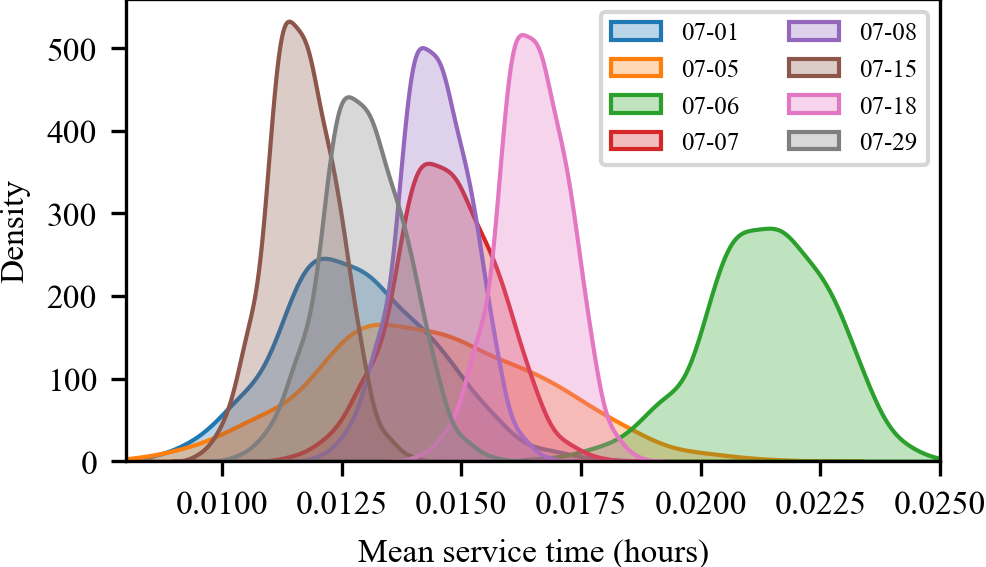
\includegraphics[width=0.8\linewidth]{media/s_phi_2019-07_selection.png}
    \caption{A selection of separate posterior approximations for individual subsamples of the full dataset, each corresponding to a single day from July 2019, as listed in the legend.}
    \label{fig:s-phi-selection}
\end{figure}


\begin{table}[htb]
    \centering
    \begin{tabular}{|c||c|c|}
        \hline
        Date & $\hat\mu$ (hrs) & $\hat\sigma$ (hrs) \\
        \hline\hline 
        2019-07-01 & 0.01283 & 0.002107 \\
        \hline
        2019-07-05 & 0.01427 & 0.002271 \\
        \hline 
        2019-07-06 & 0.02123 & 0.002229 \\
        \hline
        2019-07-07 & 0.01472 & 0.002315 \\
        \hline
        2019-07-08 & 0.01451 & 0.002305 \\
        \hline 
        2019-07-15 & 0.01181 & 0.001953 \\
        \hline
        2019-07-18 & 0.01650 & 0.002414 \\
        \hline
        2019-07-29 & 0.01305 & 0.002140 \\
        \hline
    \end{tabular}
    \caption{Estimated mean $\hat\mu$ and standard deviation $\hat\sigma$ in hours for daily posteriors $\svn$.}
    \label{tab:s-phi-selection}
\end{table}


\subsection{Final Loss Construction}

This breaks up our optimization problem into two steps. First, we wish to find individual
\begin{equation}
    \hat\psi^{(k)}, \hat\theta^{(k)} = \argmax_{\psi,\theta} \underbrace{\EX{\rz\sim\svd{\cdot\given x^{(k)};c^{(k)}, y^{(k)}}}{\log\frac{\pld{x^{(k)}\given z, y^{(k)}}\pld{z;c^{(k)}}}{\svd{z\given x^{(k)};c^{(k)}, y^{(k)}}}}  }_{\elbo{s}{\psi, \theta, x^{(k)}; c^{(k)}, y^{(k)}}}
\end{equation}
for each $(x^{(k)},w^{(k)}, y^{(k)})\in\Data$, where $c^{(k)}=\fvd{w^{(k)}}$. For clarity, we re-iterate that we have specifically learned these variational approximations $\svd{z\given y;c}$ for each $y$ and $c$, and $\svn$ does not immediately accept $y$ as an input. Also, in our case, $\theta$ as pertains to $\pld{x\given z;y}$ is assumed to be empty, so we are really just finding $\hat\psi^{(k)}$. Once we have learned these, we then approximate
\begin{equation}
    \elbo{q}{\phi,\theta,x;c,d,y}\approx \log \pld{x;c,y} - \DKL{\qvd{\cdot ; d}}{\svd{\cdot \given x;c,y}},
\end{equation}

and just use this as usual in our previously derived
\begin{equation}
    \hat\phi,\hat\theta,\hat\nu,\hat\gamma = \argmax_{\phi,\theta,\nu,\gamma} \sum_{(x,y,w)\in \Data} \elbo{q}{\phi,\theta,x;\fvd{w},\gvd{x,y,w},y}.
\end{equation}

\begin{proposition}[Final Loss Construction]
    To fit loss conventions, we negate this and instead solve the mirrored problem
    \begin{equation}
        \hat\phi,\hat\theta,\hat\nu,\hat\gamma = \argmin_{\phi,\theta,\nu,\gamma} \sum_{(x,y,w)\in \Data} -\elbo{q}{\phi,\theta,x;\fvd{w},\gvd{x,y,w},y}.
    \end{equation}    
\end{proposition}

